\section{Innledning}
\subsection{Bakgrunn for oppgaven}
Sommeren 2021 hadde Håkon sommerjobb hos Kongsberg Maritime, avd. VeRo (Vessel Robotics). 
I samråd med firmaet kom vi frem til en oppgave som kan passe oss. Kongsberg Maritime ser 
på bruken av Ultra Wide Band (UWB) til posisjonering av en ROV på siden av skip. Og i den 
forbindelse ønsket de at vi skal se på bruk av UWB posisjonering på droner.

\subsubsection{Kongsberg Maritime}
Kongsberg Maritime er en teknologibedrift som hører til Kongsberg Gruppen. 
Kongsberg gruppen stammer opprinnelig fra Kongsberg våpen fabrikk, 
men i dag er det en høyteknologisk bedrift som driver med blant annet våpen, 
romfart og maritim teknologi. Kongsberg Maritime leverer blant annet systemer 
for posisjonering, overvåking, navigasjon og automasjon til skip og offshoreinstallasjoner.

\begin{figure}[htp]
    \centering
    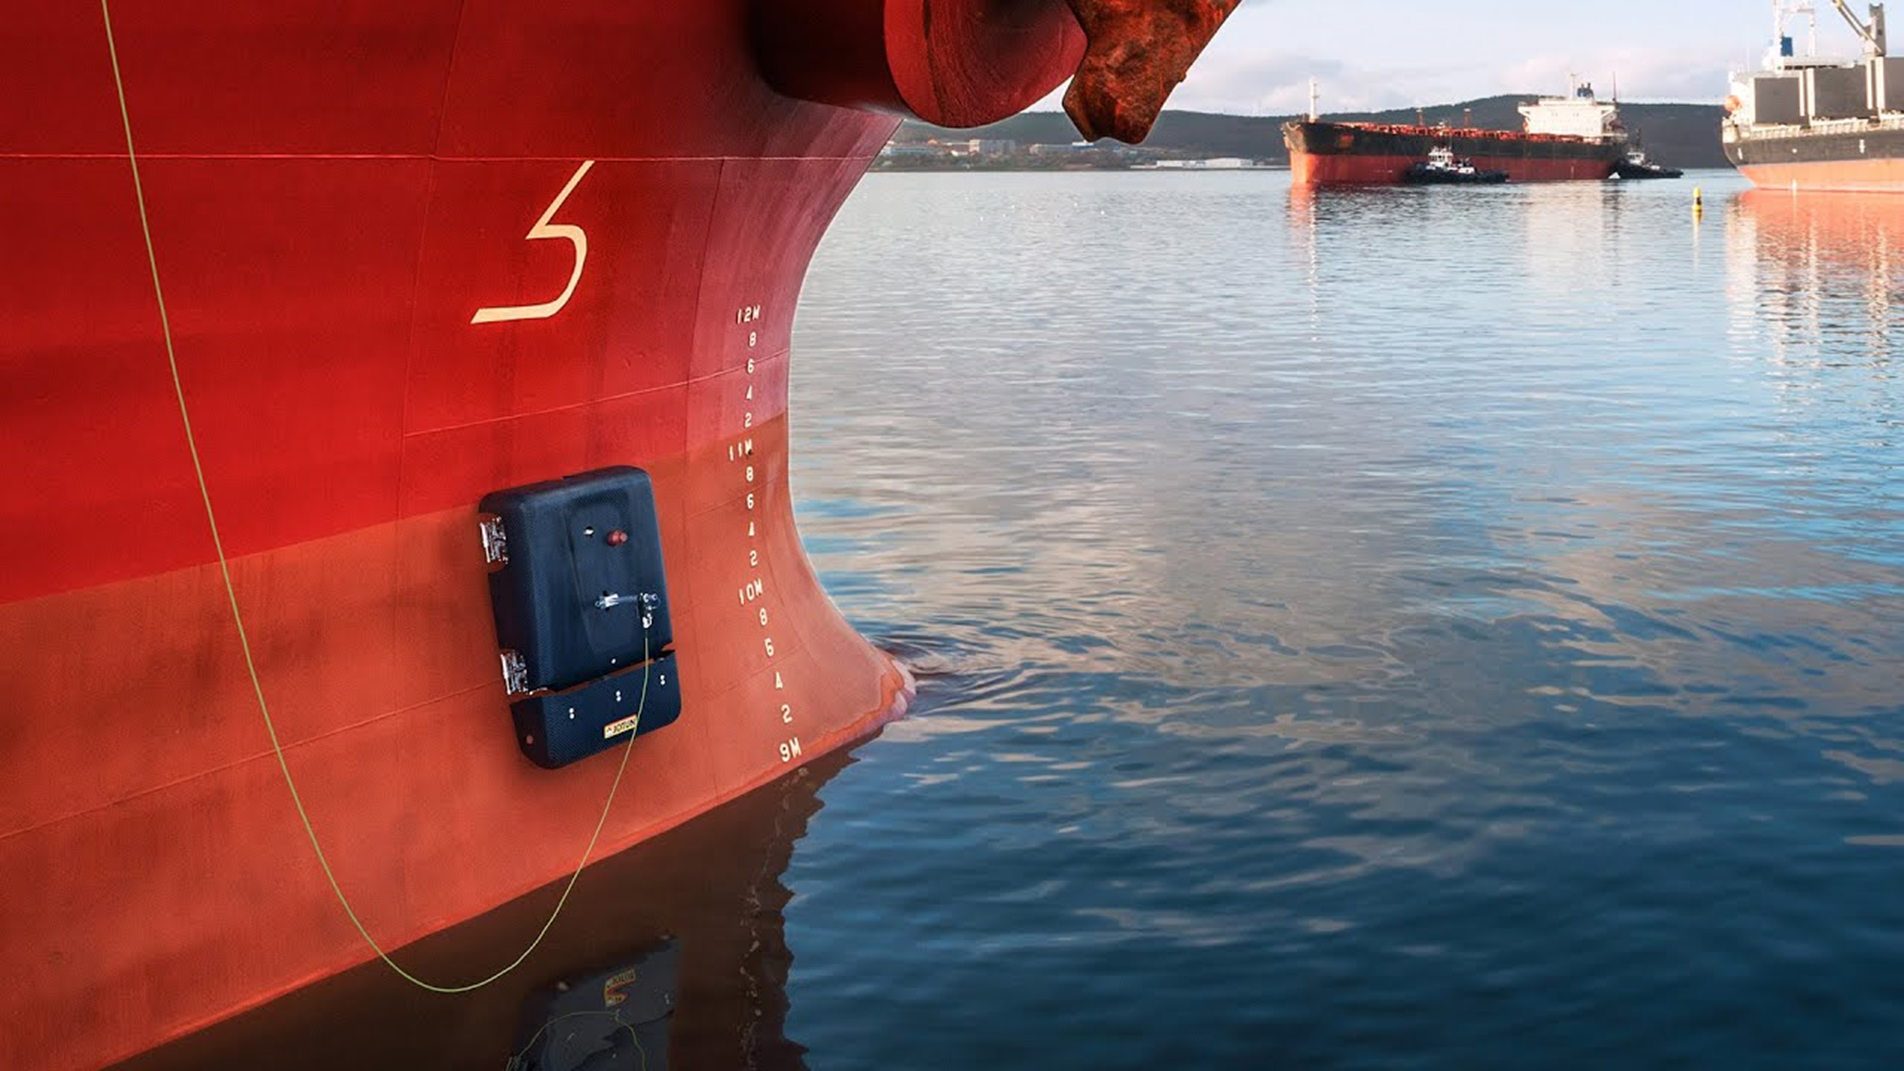
\includegraphics[width=0.7\columnwidth]{figures/hullskater}
    \caption{Hull Skater.}
    \label{fig:hullskater}
\end{figure}

Maritime har kontorer over hele verden, der hovedkontoret ligger i Norge.
HSS, Hull Skating Solutions, er et samarbeidsprosjekt mellom Jotun og Kongsberg Maritime. 
Prosjektet utvikler en robot som kan brukes til å vaske skroget på store skip. 
Dette blir gjort for å hindre uønsket spredning av organismer rundt om i verden, 
samt minke drivstofforbruket på båtene. Slik det gjøres i dag må båtene tas opp på land for å bli vasket, 
eller dykkere må dykke langs skroget for å rengjøre. 
\parencite{Keim2015}


\subsection{Problemstilling}
VeRo ønsker å vite hvor på skipskroget HullSkater befinner seg. Skipskroget er et vertikalt plan 
som står normalt på vannoverflaten. GNSS vil her ikke gi tilstrekkelig presisjon for posisjonen. Noen grunner til dette er:
\begin{itemize}
    \item GNSS gir ikke god høydepresisjon, og vil derfor bli for unøyaktig til dette bruksområdet.
    \item GNSS måler skipets og HullSkater sin posisjon i forhold til jorden.
    \item Skipet vil ikke alltid ligge like dypt i vannet.
    \item GNSS tar ikke høyde for endring i vannhøyden.
\end{itemize}
Med UWB kan man lage et lokalt posisjoneringssystem som vil fikse dette problemet og gi posisjonen til roboten på skroget uavhengig av posisjonen til skipet. 
Mangelen på lokal posisjonering er et problem som oppstår flere plasser hvor det er viktigere å vite posisjonen i forhold til en gjenstand enn plassering på jordens overflate. Eksempler på dette i forbindelse med droneaktivitet er anleggsplasser, maritime operasjoner fra plattform eller skip og inspeksjon av konstruksjoner og bygninger. 
Tidligere er det kun brukt GNSS under disse operasjonstypene. Noen problemer med GNSS i disse situasjonene er:
\begin{itemize}
    \item I forbindelse med operasjoner i urbane miljø er signalrefleksjon et stort problem. Dette gir dårligere nøyaktighet og mindre troverdig posisjon.
    \item GNSS kan lett forstyrres av andre signaler da signalet som treffer jorda er svakt i forhold til andre trådløse former for kommunikasjon.
    \item GNSS har en begrenset evne til å bestemme høyde. På grunn av plasseringen og avstanden til satellittene. 
\end{itemize}

\subsection{Målformulering}
\subsubsection{Formål}
Gruppen skal se på bruken av UWB posisjonering av dronesystemer og se på fordeler og ulemper med dette kontra GNSS.  

\subsubsection{Resultatmål}
Dette prosjektet ønsker å se på bruken av et UWB system på en drone samt å sammenlikne presisjonen med GNSS. For å oppnå dette er det i samarbeid med VeRo satt flere delmål det skal jobbes mot. Disse er laget med økende kompleksitet, da det er vanskelig å si på forhånd hvor mye hvor mye tid det vil ta å oppnå de ulike målene. Målene med UWB er:
\begin{itemize}
    \item Posisjonen til dronen blir loggført under en manuell innendørs flygning.
    \item Dronen holder automatisk posisjonen sin i luften.
    \item Dronen kan lande automatisk.
    \item Dronen kan fly et preprogrammert oppdrag med takeoff, planlagt rute og landing.
\end{itemize}
Det er veldig mange problemer med GNSS-baserte droneoperasjoner som muligens kan løses med UWB-posisjonering. Det er derfor ønskelig å utvikle et system som bruker UWB-posisjonering og undersøke hvilke muligheter med også problemer som dette gir.
Et siste mål er å sammenlikne presisjonen oppimot GNSS. Dette målet regnes som uavhengig i forhold til de andre målene.

\subsubsection{Prosessmål}
Gi studentene erfaring og kompetanse i å samarbeide i team, samt å planlegge og gjennomføre et større prosjekt.